%; whizzy chapter -dvi
% -initex iniptex -latex platex -format platex -bibtex jbibtex -fmt fmt
% 以上 whizzytex を使用する場合の設定。
 
%     Tokyo Debian Meeting resources
%     Copyright (C) 2012 Junichi Uekawa
%     Copyright (C) 2011, 2015 Nobuhiro Iwamatsu

%     This program is free software; you can redistribute it and/or modify
%     it under the terms of the GNU General Public License as published by
%     the Free Software Foundation; either version 2 of the License, or
%     (at your option) any later version.

%     This program is distributed in the hope that it will be useful,
%     but WITHOUT ANY WARRANTY; without even the implied warranty of
%     MERCHANTABILITY or FITNESS FOR A PARTICULAR PURPOSE.  See the
%     GNU General Public License for more details.

%     You should have received a copy of the GNU General Public License
%     along with this program; if not, write to the Free Software
%     Foundation, Inc., 51 Franklin St, Fifth Floor, Boston, MA  02110-1301 USA

%  preview (shell-command (concat "evince " (replace-regexp-in-string "tex$" "pdf"(buffer-file-name)) "&"))

%%ここからヘッダ開始。

\documentclass[mingoth,a4paper]{jsarticle}
\usepackage{monthlyreport}
% 日付を定義する、毎月変わります。
\newcommand{\debmtgyear}{2015}
\newcommand{\debmtgmonth}{8}
\newcommand{\debmtgdate}{22}
% started from zero:
% (let ((year 2013) (month 7)) (+ (* (- year 2005) 12) month -1))
\newcommand{\debmtgnumber}{129}

% tikz picture の為のマクロ設定
\usepackage[dvipdfmx]{graphicx}
\usepackage{tikz}

\begin{document}

\begin{titlepage}
\thispagestyle{empty}
% タイトルページ:編集必要な部分は最初のマクロに飛ばすこと

\vspace*{-2cm}
第\debmtgnumber{}回 東京エリア Debian 勉強会資料\\
\hspace*{-2cm}

\includegraphics{image2012-natsu/dotdeb.pdf}\\
\hfill{}\debmtgyear{}年\debmtgmonth{}月\debmtgdate{}日

% ここはアップデートすること
% 全角文字にしないとフォントのサイズが合わないので注意
\rotatebox{10}{\fontsize{30}{30} {\gt 特集:APT1.1 超☆牛さんパワー}}\\

\vspace*{-2cm}
\hfill{}
\includegraphics[height=6cm]{image200502/openlogo-nd.eps}
\end{titlepage}

\newpage

\begin{minipage}[b]{0.2\hsize}
 \definecolor{titleback}{gray}{0.9}
 \colorbox{titleback}{\rotatebox{90}{\fontsize{80}{80} {\gt デビアン勉強会} }}
\end{minipage}
\begin{minipage}[b]{0.8\hsize}
\hrule
\vspace{2mm}
\hrule
\begin{multicols}{2}
\tableofcontents
\end{multicols}
\vspace{2mm}
\hrule
\end{minipage}

\dancersection{事前課題}{野島 貴英}

今回の事前課題は以下です:
\begin{enumerate}
\item 本日、何の作業をやるかを宣言ください。
\item (オプション) どこで今回の勉強会の開催を知りましたか?
\item (オプション) 何について聞きたい/参加者と話をしたいですか?
\end{enumerate}
この課題に対して提出いただいた内容は以下です。
\begin{multicols}{2}
{\small
\begin{prework}{ 野島 }
  \begin{enumerate}
  \item Q.hack timeに何をしますか?\\
    A. 今度こそ!Nook HD+をDebianに。
  \item (オプション)Q.何について聞きたい/参加者と話をしたいですか?\\
    A. 俺とDebian
  \end{enumerate}
\end{prework}

\begin{prework}{ zinrai }
  \begin{enumerate}
  \item Q.hack timeに何をしますか?\\
    A. mincsのITP。https://github.com/mhiramat/mincs
  \end{enumerate}
\end{prework}

\begin{prework}{ wskoka }
  \begin{enumerate}
  \item Q.hack timeに何をしますか?\\
    A. tilegxへの移植
  \item (オプション)Q.どこで今回の勉強会の開催を知りましたか?\\
    A. その他
  \end{enumerate}
\end{prework}

\begin{prework}{ issei }
  \begin{enumerate}
  \item Q.hack timeに何をしますか?\\
    A. dgitの使い方をマスターする。
  \end{enumerate}
\end{prework}

\begin{prework}{ khibino }
  \begin{enumerate}
  \item Q.hack timeに何をしますか?\\
    A. Debian haskell チームへの参加について調べる
  \item (オプション)Q.どこで今回の勉強会の開催を知りましたか?\\
    A. 友達や知り合いから直接
  \end{enumerate}
\end{prework}

\begin{prework}{ Roger Shimizu }
  \begin{enumerate}
  \item Q.hack timeに何をしますか?\\
    A. Debian BTSの確認など
  \item (オプション)Q.どこで今回の勉強会の開催を知りましたか?\\
    A. その他
  \end{enumerate}
\end{prework}


\begin{prework}{yy\_y\_ja\_jp}
  \begin{enumerate}
  \item Q.hack timeに何をしますか?\\
    A. DDTSS\\
    http://ddtp.debian.net/ddtss/index.cgi/ja
  \item (オプション)Q.何について聞きたい/参加者と話をしたいですか?\\
    A. DDTSS
  \item (オプション)Q.どこで今回の勉強会の開催を知りましたか?\\
    A. その他
  \end{enumerate}
\end{prework}



}
\end{multicols}

\dancersection{最近のDebian関連のミーティング報告}{野島 貴英}

\subsection{第128回東京エリアDebian勉強会}

\begin{itemize}
\item 場所はスクウェア・エニックスさんのセミナルームをお借りしての開催でした。
\item 参加者は6名でした。
\item セミナ内容は野島さんによる「DebianでHTTP/2を試す」でした。
\item 残りの時間でhack timeを行い、成果発表をしました。
\item 宴会の代わりに、「中国料理 東順永 本店」で夕食会をやりました。
\end{itemize} 

 セミナは野島さんより、DebianでHTTP/2を試す事について発表がありました。内容としては、HTTP/2の規格概要、デモ、Debianで最も簡単にHTTP/2対応サーバを動かしてみる等となりました。今年RFC化される、あるいは、某有名携帯端末の会社のイベントでHTTP/2を使って欲しいアピールがあったなど、HTTP/2が少しづつ推される(あるいはいつの間にか使っている?)場面も、今後増えてくるかと思います。Debianがあればサーバ稼働も含めてすぐに試せますので、皆様も是非お試し下さい。

 また、参加者の中で、hacktime中に書いたLinux Kernel向けパッチが取り込まれた、Bug Reportした内容がLWN/Gigazineに取り上げられた等、いろいろな形で成果を出された旨の報告がありました。こういった方々がいらっしゃるのは正直凄い事だと思います。

 Debianは多様性をモットーとしているコミュニティでもあります。参加したいと思った方々には、IT技術面・非IT技術面、どちらも十分に活躍して成果をうたえる余地にあふれ、万年人手不足のコミュニティです。参加された方々におきましては、様々な形でいつでも頭角を表していただけるチャンスにあふれてますので、皆様も是非!

% % (query-replace-regexp "<.*?>" "")
% % (query-replace-regexp "^[	 ]\+" "")

%-------------------------------------------------------------------------------
\dancersection{APT1.1 超☆牛さんパワー炸裂!}{野島 貴英}
%-------------------------------------------------------------------------------

\subsection{はじめに}

 debian-devel-announceに、''Moo! 9th preview of APT 1.1 released: Go and test new supercow powers''というタイトルで、APT 1.1のアナウンスが流れました。

 今回は、Debianの重要なツールの1つであるAPTについて、1.1に搭載された特徴をネタにして、いろいろ調べてみました。

\subsection{Debconf15のセッション}

 2015/8/15-8/22で開催されたDebconf15のセッションで、APT1.1のセッションが開かれました。こちらビデオが公開されていますので、興味ある方は是非ご覧ください。

 ビデオ:''This\_APT\_has\_Super\_Cow\_Powers''\\
 \url{http://meetings-archive.debian.net/pub/debian-meetings/2015/debconf15/This_APT_has_Super_Cow_Powers.webm}

\begin{figure}[H]
\begin{center}
 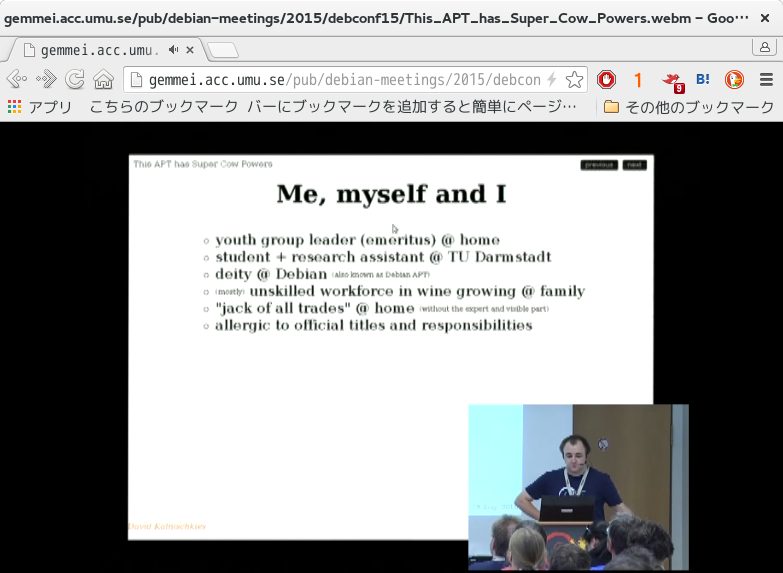
\includegraphics[width=0.5\hsize]{image201508/debconf15-apt.png}
\end{center}
\caption{Debconf15のAPT1.1のセッションの様子}
\end{figure}

\subsection{APT 1.1を評価してみる}

 2015/8/22現在、APT 1.1はexperimentalリポジトリにあります。早速、試して見たい方は以下のようにすることで導入できます。

\begin{commandline}
$ sudo vi /etc/apt/source.lists
deb http://ftp.jp.debian.org/debian/ experimental main contrib non-free
deb-src http://ftp.jp.debian.org/debian/ experimental main contrib non-free
$ sudo apt-get update
$ sudo apt-get -t experimental install apt
$ apt
apt 1.1~exp9 (amd64)
Usage: apt [options] command
...中略...
 full-upgrade - upgrade the system by removing/installing/upgrading packages
 edit-sources - edit the source information file
\end{commandline}

 手元のDebian sid環境に導入してしばらく使っていますが、特に動作に問題は見当たりませんでした。apt update,apt full-upgrade, apt autoremoveなど一通りの動作は問題なくできており、致命的なバグにも特に遭遇していません。是非お試しあれ。

\subsection{APT 1.1の特徴}

 jessie搭載のAPT 1.0.9.8に比べての違いを述べてみます。

 先に紹介したDebconf15のビデオによれば以下の点が違いとなります。

\begin{itemize}
\item リポジトリの情報のセキュリティ検証が強化された。
\item deb822形式でリポジトリを指定するやり方にて機能強化。(/etc/apt/*.sourcesファイル)
\item httpredir.debian.orgを受けて、処理の途中経過の表示を変更。
\item Pinningがちゃんと動くようになった。
\item 依存関係をする場合、ローカルにおいた.debファイルを直接指定してもインストールでき、ソースビルドの依存関係を指定する方法が柔軟になった。
\end{itemize}

 まずは、man apt、man apt-getで記載されている内容で、トピックを絞って違いを紹介します。

\subsubsection{apt autoremove}

 APT1.1に搭載されたaptコマンドのautoremove命令について説明します。

 何かパッケージをインストールした場合、依存関係を満たすためだけにインストールされたパッケージが過去にあるとします。ここで、現在はその依存関係からも外されており、もはや全く使われていないパッケージがあります。このコマンドをつけてaptコマンドを起動すると、こういった使われていないパッケージを削除することが出来ます。

\begin{commandline}
$ sudo apt autoremove
\end{commandline}
%$

\subsubsection{autoremove仕組み}

 autoremoveはどのようにして消去すべきパッケージを見つけるのでしょうか?

 依存関係が見当たらないパッケージの中には、利用者が自分で明示して入れたパッケージもあります。そのため、必ずしも他のパッケージで依存していないということだけを条件にして、autoremoveでパッケージを消すようなことは避けなければなりません。autoremoveにより、自動で消去して良いパッケージを判断する基準は次の通りです。
 
\begin{description}
 \item [Step 1.] /var/lib/apt/extended\_statesファイルの記録に、過去、依存関係を満たすためにパッケージを導入したかどうかの記録である''Auto-Installed: 1''と記されているパッケージを消去の候補とする。
 \item [Step 2.] すでにインストール済パッケージのどれからも依存関係に無いかどうか?
 \item [Step 3.] さらに、
\begin{itemize}
\item Recommendsとして提案されているパッケージはインストールして欲しいと明示した場合、
\item Suggestとして提案されているパッケージはインストールして欲しいと明示した場合、
\end{itemize}
のいずれにも該当していないか?
\end{description}

以上のStep 1.〜3.の判断を経たパッケージが、自動で消去して良いパッケージとして扱われます。

\subsubsection{man apt-getとの違い}

次にman apt-getで見た1.0.9.8との違いについて紹介します。

 \begin{itemize}
\item indextargets \\
   apt-get updateで更新されるファイルと状態をdeb822形式で表示します。
 \item --allow-downgrades \\
   特定パッケージをダウングレードすることにより依存関係が満たせるときに、ユーザに尋ねず実行してまうというオプションです。
 \item --allow-remove-essential \\
   何らかの理由によりDebianシステムの必須パッケージ(essentialパッケージとして分類されている)ものを消せば依存関係が満たせるときに、消してよいか?を尋ねず消してしまうオプションです。
 \item --allow-change-held-packages \\
  何らかの理由によりHold扱いにしたパッケージを削除すれば依存関係が満たせるときに、消してよいか?を尋ねず消してしまうオプションです。
 \item --no-allow-insecure-repositories \\
   リポジトリにあるReleaseファイル(InReleaseファイル)のGPGによる署名が確認出来ない等、セキュリティ上問題があるとみなされたリポジトリが含まれた場合、apt-get update操作を失敗させます。
 \end{itemize}
 
 \subsubsection{リポジトリ堅牢化}

 APT 1.1はリポジトリのセキュリティの正当性評価が強化されています。正当性評価の元となるファイルにReleaseファイル(InReleaseファイル)があります。

\begin{commandline}
$ curl http://cloudfront.debian.net/debian/dists/unstable/InRelease
-----BEGIN PGP SIGNED MESSAGE-----
Hash: SHA256

Origin: Debian
Label: Debian
...中略...
MD5Sum:
 e9f9b477f2430a7d0e2dd686da1af507 30975818 Contents-amd64.gz
 d158f809191a841bedf9ff50e34e0ebe 30421142 Contents-armel.gz
...中略...
-----BEGIN PGP SIGNATURE-----
Version: GnuPG v1

iQIcBAEBCAAGBQJV1+IMAAoJEItIrWJGklVTgloP/0+XAch/TMtTSfH+N1QFl+q2
Woas1LpWhHDO12U6vuPq5wghCPYE5ctNuDxFtTy9j01lsf6kWXPDh1QupNENDNHr
lfZ7Qa9gFr8W3tH1tnPwsSqcQmu9bMkR0sRDVSfcFlDioVhN/h+jWW7j7J7nrZrE
...中略...
\end{commandline}
   
InReleaseファイルを見るとわかるとおり、

\begin{itemize}
\item リポジトリに含まれる様々なファイルは全てmd5sum付きでInReleaseファイルに記録
\item さらにInReleaseファイルも電子署名による正当性確認が出来るようになっている
\end{itemize}

となります。

 今回APT1.1では、基本的にInReleaseファイルの無い、あるいは、他に必要なファイルが欠落しているなど、セキュリティ観点からの正当性確認が出来ないリポジトリは取り扱いを完全にやめる設計にしたとのことです。

\subsubsection{httpredir.debian.org対応}

 2015/5月頃、Debianユーザに最も近いmirrorサーバーをHTTP Redirectでaptに教えてくれるサービスが稼働しました。つまり、ユーザは/etc/apt/sources.listに、httpredir.debian.orgを指定すれば、ユーザに最も近いmirrorサーバーへリダイレクトされます。

 ここで、リダイレクトされた結果どこのサーバから取得するのか?がわかると便利な事が多いです。このため、APT1.1のapt/apt-getはリダイレクトされた先の情報を表示するように変更されました。

\subsubsection{参考:httpredir.debian.orgの様子}

 httpredir.debian.orgが何を返却するのかを以下に示します。

\begin{commandline}
$curl -v http://httpredir.debian.org/debian/dists/sid/InRelease
> GET /debian/dists/sid/InRelease HTTP/1.1
> Host: httpredir.debian.org
> User-Agent: curl/7.44.0
> Accept: */*
> 
< HTTP/1.1 302 Found
< Date: Sat, 22 Aug 2015 03:54:12 GMT
< Location: http://cloudfront.debian.net/debian/dists/sid/InRelease
< Content-Type: text/plain
...省略...
\end{commandline}    

 見てのとおり、cloudfront.debian.netにリダイレクトが指示されるのが確認できると思います。

{ \scriptsize
 \begin{itembox}[l]{cloudfront.debian.net?}
 前ページのリダイレクト先にて、
\url{http://cloudfront.debian.net/}
とリポジトリが提案されています。これは、2年前にdebian-cloudチームでアナウンスがあった、AWSのcloudfrontというCDNの仕組みを使ってデータ配布を行う試みのリポジトリです。
(\url{https://lists.debian.org/debian-cloud/2013/05/msg00066.html})

 もともと、CDNはユーザに最も効率的なサーバを提示してデータを配る仕組みであり、
AWSのcloudfrontは相当な規模とサービスエリアを持つCDNサービスですので、
そもそもこちらがあるなら、AWSのサービスがカバーしている国では、httpredir.debian.orgを使わなくてすみそうな気もします。しかしながら、ソフトウェア自由をモットーとするDebianとしては、一企業のサービスに依存しないようにすることが重要ですので、Debianとしては、httpredir.debian.orgを維持・運用する必要があります。
 \end{itembox}
}

\subsection{deb822形式}

 APT 1.1では、deb822形式でリポジトリを指定するやり方にて機能強化が図られました。ここでは、deb822形式とはどんなものかを紹介します。

 APT1.1が手元にあれば、簡単にdeb822形式でリポジトリの情報を表示させる事が出来ます。

\begin{commandline}  
$ apt-get indextargets
MetaKey: main/source/Sources
ShortDesc: Sources
Description: http://ftp.jp.debian.org/debian sid/main Sources
URI: http://ftp.jp.debian.org/debian/dists/sid/main/source/Sources
Filename: /var/lib/apt/lists/ftp.jp.debian.org_debian_dists_sid_main_source_Sources
Optional: no
Codename: sid
...中略...
\end{commandline}  
  
 出力されるフォーマットを見るとわかるのですが、RFC822ヘッダの形式によく似ています。ここから、deb822と名前を取ったようです。

  特徴として、RFC822と同様ですので、ヘッダを増やせば、簡単に機能拡張できるという点が上げられます。

  また、動作未確認ですが、DebConf15のビデオによれば、
\begin{quote}
  /etc/apt/source.list.d/xxxx.sources
\end{quote}
(末尾が、.sourcesである事が必要)という名前でdeb822形式で置いておくと、
こちらをsources.listに指定したのと同様の動作をapt/apt-getは行う都のことです。
  
\subsection{牛さんパワー健在!}

 APT 1.1にも''moo''命令は健在です。息抜きに、こちらを紹介しておきます。

 man aptには記載の無いオプションですが、以下にaptの場合の起動方法を載せます。

\begin{commandline}  
$ apt moo 
$ apt moo moo [--color]
$ apt moo moo moo  
$ faketime '1997-04-01' apt moo
\end{commandline}    

\begin{figure}[H]
\begin{center}
 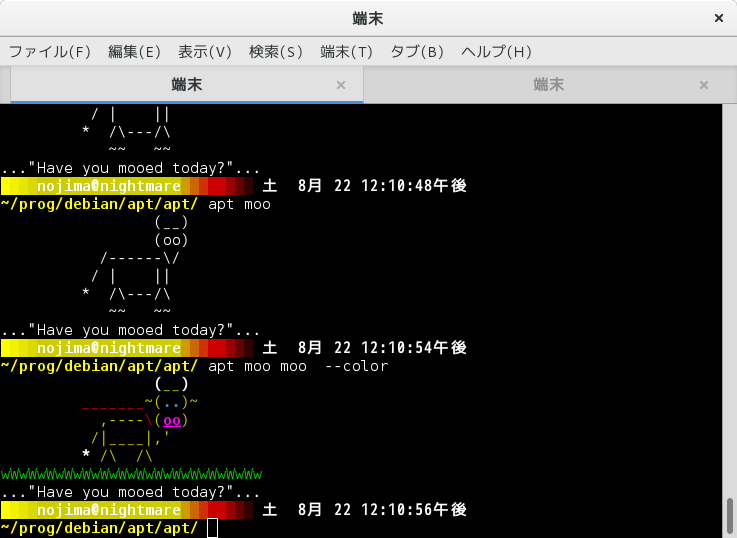
\includegraphics[width=0.7\hsize]{image201508/apt-moo.png}
\end{center}
\caption{apt mooコマンド結果例}
\end{figure}

 実行するとわかるのですが、ASCIIキャラクタで描画された各種の牛の絵が表示されます。

\subsection{おわりに}

 まだまだ、APT1.1について、今回ここでは書ききれない程の変更が加えられているようですが、このへんにしておきます。実際、gitで落として差分を確認しましたが、実に2万行を超える変更が行われていました。正式リリースになって、ドキュメントも充実すると良いですね。
   
%-------------------------------------------------------------------------------
\dancersection{会場での無線LANのつなぎ方}{野島 貴英,Roger}
%-------------------------------------------------------------------------------
 \subsection{はじめに}

 今回試験として、会場側でフィルタ無しのグローバル回線を用意しました。
ただ、会場側のセキュリティポリシーにより、wpa-psk AES hidden SSIDという
方式での提供となります。

 以下にDebianマシンでの接続方法を記載します。

 また、自分の環境では違うやり方でつながったという方は、野島まで
教えて下さい。こちらでもノウハウとして溜めていく予定です。

 \subsection{wpasupplicant及び/etc/network/interfacesを利用の場合}

 もっとも良いマニュアルは、/usr/share/doc/wpasupplicant/README.Debian.gz
となります。困った場合はこちらも合わせてご参照下さい。

 以下に/etc/network/interfacesの定義について会場の例を記載します。

\begin{commandline}
$ sudo vi /etc/network/interfaces
-----以下のエントリがなければ追記ここから----------
iface wlan0_debian inet dhcp
     wpa-conf /etc/wpa_supplicant/wpa_supplicant_debian.conf
-----以下のエントリがなければ追記ここまで----------
$ sudo vi /etc/wpa_supplicant/wpa_supplicant_debian.conf
-----以下のエントリを追記ここから----------
network={
     ssid=<<会場のSSID>>
     psk=<<会場のパスワード>>
     scan_ssid=1
}
-----以下のエントリを追記ここまで----------
$ sudo chmod 600 /etc/wpa_supplicant/wpa_supplicant_debian.conf
$ sudo ifup wlan0=wlan0_debian
\end{commandline}
%$

 また、ハマってしまった時のデバッグ方法は、
/usr/share/doc/wpasupplicant/README.Debian.gz中の''4. Trubleshooting''の章が便利です。

 \subsection{その他の無線LAN用パッケージを利用の場合}

 すみません、自分が情報を持たないため、現場で教えて下さい。

\cleartooddpage

\vspace*{15cm}
\hrule
\vspace{2mm}

\includegraphics[width=2cm]{image200502/openlogo-nd.eps}
\noindent \Large \bf Debian 勉強会資料\\
\noindent \normalfont \debmtgyear{}年\debmtgmonth{}月\debmtgdate{}日 \hspace{5mm}  初版第1刷発行\\
\noindent \normalfont 東京エリア Debian 勉強会 (編集・印刷・発行)\\
\hrule

\end{document}
